\chapter{Implementierung}
\label{ch:Implementierung}

\section{Hostsystem}
\label{sec:Hostsystem}

\subsection{Grundkonfiguration}
\label{subsec:Grundkonfiguration}

Als Hostsystem kommt ein Debian Jessy (Version 8.6) 64-Bit zum Einsatz. Dieses System ist ein virtuelles System, welches auch als vServer bezeichnet wird. Bereitgestellt wird dieser vServer von providerdienste.de\footnote{\url{https://www.providerdienste.de/}} mit folgenden Eigenschaften:

\begin{itemize}
\item 2 CPU-Kerne a 2,67 GHz
\item 2 GB Arbeitsspeicher
\item 50 GB Festplatte
\item 1 IPv4-Adresse
%\item 10 Ipv6-Adressen
\end{itemize}

Das System wurde mit diesen Eigenschaften gewählt, um sicherzustellen, dass für diesen Versuchsaufbau ausreichend Rechenleistung und Speicher zu Verfügung steht. Zudem ist die öffentliche IPv4-Adresse zu nennen, die den Teammitgliedern in einem Versuchsaufbau in einem privaten Heimnetzwerk aus technischen Gründen nicht zur Verfügung gestanden hat. Die Verwaltung des Servers erfolgt zunächst über SSH über einen Root-Zugang, der von providerdienste.de bereitgestellt wird.
Alternative ist eine Verwaltung über eine sogenannte Remote-Konsole möglich. Über diese Konsole  kann das System jederzeit gestartet und gestoppt werden oder auch das root-Passwort neu gesetzt werden, selbst dann wenn kein Zugriff via SSH zu Verfügung steht. Zudem kann eine Neuinstallation ausgeführt werden.\\

Da das System als installiertes System mit funktionsfähiger Netzwehrkonfiguration übergeben wurde, ist der erste Schritt eine Aktualisierung der installierten Pakete. Dazu werden die Paketlisten neu eingelesen und neue Paketversionen installiert:

\begin{lstlisting}[style=customc]
apt-get update && apt-get dist-upgrade
\end{lstlisting}

Um nicht ausschließlich mit root-Rechten zu arbeiten wird für jedes Teammitglied ein eigener Benutzer mit Homeverzeichnis eingerichtet und ein vordefiniertes Passwort gesetzt:

\begin{lstlisting}[style=customc]
useradd -d /home/mstroh -s /bin/bash -m mstroh
passwd mstroh
useradd -d /home/dschwenk -s /bin/bash -m dschwenk
passwd dschwenk
\end{lstlisting}

Wird bei der Installation von Debian ein root-Passwort angegeben, wird das Programm \textit{sudo} nicht installiert. Dies ist bei dem uns vorliegen vServer der Fall. Um den Benutzern ohne den Wechsel zum Benutzer root die Ausführung von Programmen mit privilegierten Berechtigungen zu ermöglichen, wird das Programm \textit{sudo} über \textit{apt-get install sudo} installiert. Die Benutzer werden in die Gruppe \textit{sudo} aufgenommen:

\begin{lstlisting}[style=customc]
adduser mstroh sudo
adduser dschwenk sudo
\end{lstlisting}

Zudem müssen die Benutzer in die Datei /etc/sudoers aufgenommen werden:

\begin{lstlisting}[style=customc]
dschwenk ALL=(ALL:ALL) ALL
mstroh ALL=(ALL:ALL) ALL
\end{lstlisting}

Die Benutzer können somit über \textit{sudo} Aktionen, für die privligierte Berechtigungen notwendig sind, durchführen. Damit ist die Grundkonfiguration des vServers abgeschlossen. %TODO .. wirklich? fehlt  noch was?


\subsection{Konfiguration Serverdienste}
\label{subsec:Konfiguration Serverdienste}

Das System wurde von providerdienste.de mit einem aktiven SSH-Dienst ausgeliefert. Da der Login eines root-Benutzers über SSH aus Sicherheitsgründen vermieden werden sollte, wird nachfolgend eine Public-Key-Authentifizierung für die Benutzeraccounts der Teammitglieder konfiguriert.\\

Damit eine Public-Key-Authentifizieurng stattfinden kann, muss im jeweiligen Benutzerverzeichnis auf dem Server ein \textit{.ssh}-Verzeichnis mit entsprechenden Berechtigungen angelegt werden.

\begin{lstlisting}[style=customc]
mkdir ~/.ssh
chmod 700 ~/.ssh
\end{lstlisting}

Auf dem lokalen System der Teammitglieder wird jeweils das Schlüsselpaar erzeugt:

\begin{lstlisting}[style=customc]
ssh-keygen -t rsa -C "Kommentar"
\end{lstlisting}

In das oben erzeugte \textit{.ssh}-Verzeichnis wird jeweils der öffentliche Schlüssel in die Datei \textit{authorized\_keys} abegelegt:

\begin{lstlisting}[style=customc]
cat id_dsa.pub | ssh username@server 'cat >> .ssh/authorized_keys'
\end{lstlisting}

Die Berechtigungen auf die Datei \textit{authorized\_keys} wird jeweils über \textit{chmod 600 ~/.ssh/authorized\_keys} angepasst.\\

Um die Authentifizierung via Passwort zu deaktivieren wird die die \textit{sshd\_config} unter \textit{/etc/ssh/} wie folgt angepasst:

\begin{lstlisting}[style=customc]
ChallengeResponseAuthentication no
PasswordAuthentication no
UsePAM no
\end{lstlisting}

Ebenfalls wird der Parameter \textit{PermitRootLogin} auf \textit{no} gesetzt, um einen zukünftigen Login des root-Benutzers zu deaktivieren. Abschließend wird der SSH-Dienst mit einem

\begin{lstlisting}[style=customc]
/etc/init.d/ssh restart
\end{lstlisting}

neu gestartet. Von nun an ist nur noch eine Anmeldung über die Benutzeraccounts der Teammitglieder in Kombination mit einer Public-Key-Authentifizierung möglich.

\section{SSH-Honeypot}
\label{sec:SSH-Honeypot}

\subsection{Installation und Konfiguration Kippo}
\label{subsec:Installation und Konfiguration Kippo}

% vorgehenseise installation + konfiguration kippo\\
% http://www.blackhat.pm/ssh-honeypot-on-debian-with-kippo.html
% https://technik.blogbasis.net/kippo-ssh-honeypot-installieren-17-10-2014

% ausführliche Beschreibung Kippo + Dateien\\
% http://resources.infosecinstitute.com/tracking-attackers-honeypot-part-2-kippo/

Dieses Kapitel beschreibt die Vorgehensweise zur Installation und Konfiguration von einem SSH-Honeypot auf Basis von Kippo. Dieser SSH-Honeypot soll wie für SSH üblich auf Port 22 eingerichtet werden. Da aktuell der standard SSH-Dienst auf Port 22 läuft, muss dieser zuvor angepasst werden. Dazu wird der Port in der Konfigurationsdatei \textit{etc/ssh/sshd\_config} auf Port 10022 abgeändert und der Dienst anschließend neu gestartet.\\

Damit Kippo lauffähig ist, sind einige zusätzliche Pakete notwendig\footnote{ Kippo Abhängigkeiten: \url{https://github.com/desaster/kippo\#requirements}}. Diese werden, ebenso wie der git-Client für einen einfachen Download des Kippo-Projekts, installiert:

\begin{lstlisting}[style=customc]
apt-get install python-dev openssl python-openssl python-pyasn1 
  python-twisted git
\end{lstlisting}

Einer Ausführung von Befehlen oder Diensten mit root-Rechten sollte stets wohl bedacht sein und nach Möglichkeit vermieden werden. Die Ausführung des Honeypot-SSH-Dienstes mit root-Rechten oder auch unter einem unserer Benutzer wäre höchst sicherheitskritisch. Ein Angreifer könnte darüber volle Kontrolle über das Hostsystem erlangen. Um diese Gefahr möglichst gering zu halten wird ein separater Benutzer eingerichtet:

\begin{lstlisting}[style=customc]
useradd -d /home/kippo -s /bin/bash -m kippo -g sudo
\end{lstlisting}

Um auf einem Linux-System einen Port kleiner 1024 ("`well known ports"') zu verwenden sind root-Rechte erforderlich. Genau dies soll für den SSH-Honeypot-Dienst wie oben beschrieben vermieden werden. Um auch einem normalen Benutzer die Verwendung eines Ports kleiner 1024 zu ermöglichen, wird auf das Programm \textit{AuthBind}\footnote{ \textit{AuthBind}: \url{http://man.cx/authbind(1)}} zurückgegriffen. Die Installation von Authbind erfolgt via:

\begin{lstlisting}[style=customc]
apt-get install authbind
\end{lstlisting}

Die Verwendung von Port 22 wird über die Erstellung einer Datei unter \textit{/etc/authbind/byport/} sowie die Anpassung der Berechtigungen für den Kippo-Benutzer auf diese Datei ermöglicht:

\begin{lstlisting}[style=customc]
touch /etc/authbind/byport/22
chown kippo /etc/authbind/byport/22
chmod 777 /etc/authbind/byport/22
\end{lstlisting}

Der Download von Kippo erfolgt direkt von der Projektseite auf Github\footnote{ \textit{Kippo-Projekt auf Github}: \url{https://github.com/desaster/kippo}}:

\begin{lstlisting}[style=customc]
git clone https://github.com/desaster/kippo.git
\end{lstlisting}

Im Kippo-Verzeichnis befindet sich eine Datei, die eine Standardkonfiguration enthält. In dieser wird der  voreingestellte Port auf Port 22 abgeändert. Zudem muss die Konfigurationsdatei in \textit{kippo.cfg} umbenannt werden:

\begin{lstlisting}[style=customc]
mv kippo.cfg.dist kippo.cfg
\end{lstlisting}

Damit Kippo mit Hilfe von AuthBind ausgeführt wird, muss das "`Kippo-Start-Skript"' angepasst werden. Dazu wird der Befehl \textit{authbind} in das Skript aufgenommen:

\begin{lstlisting}[style=customc]
authbind --deep twistd -y kippo.tac -l log/kippo.log --pidfile kippo.pid
\end{lstlisting}

Der Parameter \textit{--deep} sorgt dafür, dass nicht nur das direkt folgende Programm, sondern auch alle Programme die folge dieses Aufrufs sind, unter \textit{authbind} ausgeführt werden. Kippo selbst basiert auf Twisted, einer "`Event-basierten Netzwerkengine"'\footnote{ \textit{Twisted - Building the engine of your internet}: \url{http://twistedmatrix.com/trac/}} für Python. twistd\footnote{ \textit{twistd}: \url{https://linux.die.net/man/1/twistd}} wird über den Parameter "`\textit{y}"' die Python-Applikation, zudem eine Logdatei sowie ein Pidfile übergeben. In diesem wird die Prozess-ID abgelegt.

Nach Ausführung des Kippo-Startskript \textit{start.sh} läuft der Prozess im Hintergrund. In Folge dessen wird auch das Kippo-Logfile angelegt, in dem Zugriffe auf den SSH-Honeypot-Dienst dokumentiert werden. Änderungen in diesem Logfile können über

\begin{lstlisting}[style=customc]
tail -f /home/kippo/kippo/log/
\end{lstlisting}

direkt verfolgt werden. Von nun an kann auch eine Verbindung auf Port 22 aufgebaut werden. Nicht zu vergessen ist, dass der SSH-Dienst auf Port 10022, der die Verbindung der Projektmitarbeiter ermöglicht, durch einen Portscanner wie NMap aufgespürt werden kann.

\begin{figure}[ht]
	\centering
		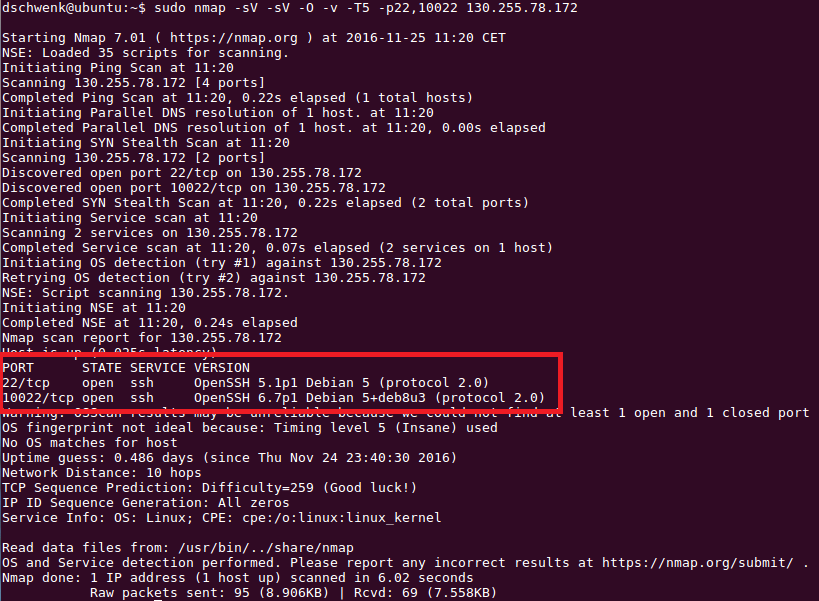
\includegraphics[width=1.0\textwidth]{img/nmap_ssh.png}
	\caption{Ausgabe Portscanner Nmap gegen das Honeypot-System}
	\label{fig:nmap_ssh}
\end{figure}

Das Kippo-SSH-Banner, welches in Abbildung \ref{fig:nmap_ssh} zu erkennen ist, kann über die Kippo-Konfigurationsdatei \textit{kippo.cfg} angepasst werden. In dieser Konfigurationsdatei können ebenfalls unter anderem folgende Einstellungen vorgenommen werden:

\begin{itemize}
\item Verzeichnis, in die Kippo eine Logdatei mit allen Aktivitäten schreibt. Alternativ kann eine Datenbank zur Protokollierung verwendet werden. Aus Zeit- und Performancegründen entscheidet sich das Projektteam für die Logdatei.
\item Angabe des Verzeichnisses, in dem die Datei \textit{fs.pickle} mit dem virtuellen Dateisystem liegt
\item Angabe einer Datei, die vordefinierten Antworten auf diverse Kommandos enthält. Die Ausgabe dieser Antworten erhält ein Angreifer nach einem erfolgreichen Login bei der Eingabe von Standardkommandos
\end{itemize}

Die Kombinationen an Benutzernamen und Passwörter, mit denen ein Login über den SSH-Honeypot möglich ist, kann in der Datei \textit{userdb.txt} spezifiziert werden. Standardmäßig ist hier der Benutzername \textit{root} mit dem Passwort \textit{123456} hinterlegt. Um einem Angreifer eine größere Angriffsfläche zu bieten, wird diese List um folgende Einträge ergänzt:

\begin{lstlisting}[style=customc]
root:123456
root:root
root:r00t
admin:123456
admin:admin
admin:password
\end{lstlisting}

Damit ist die Installation und grundlegende Konfiguration des SSH-Honeypots abgeschlossen.

\subsection{Kippo-Logfile auswerten}
\label{subsec:Kippo-Logfile auswerten}

% - extract uniq ips aus kippo logfile \\
% https://bruteforce.gr/extracting-unique-ips-from-logfile.html \\

Die IP-Adressen von Angreifern werden im Kippo.log-Logfile neben zahlreichen Informationen wie eingegeben Benutzernamen, Passwörter und Befehle gespeichert. Ein Auszug aus einem Kippo-Logfile ist im Anhang unter \textit{\nameref{app:Ausschnitt aus Kippo-Logdatei}} zu finden. Aus diesen Informationen sollen Statistiken zu Benutzernamen und Passwörter sowie automatisiert Firewallregeln erstellt werden, um Angriffe von diesen IPs zu verhindern.

Wie dem Kippo-Logfile unter \textit{\nameref{app:Ausschnitt aus Kippo-Logdatei}} zu entnehmen ist, werden Benutzernamen und Passwörter als Teile von Zeichenketten im Logfile abgelegt. Für eine Auswertung müssen diese aus dem Logfile extrahiert werden. Dies erfolgt mit Hilfe der Werkzeuge \textit{grep} und \textit{awk}. Duplikate werden durch \textit{sort} und \textit{uniq} entfernt.


% http://bob.k6rtm.net/kippowho.html

\begin{lstlisting}[style=customc]
grep ' login attempt ' kippo.log |
  awk '{print ($9)}' |
  sort |
  uniq |
  sed -r 's/]|\[//g' > user.txt

\end{lstlisting}

Hierdurch erhalten wir eine Liste von Kombinationen aus Benutzernamen und Passwörter in der Form \textit{username/passwort}. Passwörter werden zudem separat ohne Benutzernamen extrahiert. Passwortduplikate werden hierbei nicht entfernt, um daraus aussagekräftige Statistiken generieren zu können.

\begin{lstlisting}[style=customc]
grep ' login attempt ' kippo.log |
  awk '{print ($9)}' |
  sed "s|^.*/||g" |
  sed "s|]||g" > pw.txt
\end{lstlisting}

Die Ausführung dieser Befehle wird über ein Bash-Skript realisiert. Das vollständige Skript ist im Anhang unter \textit{\nameref{app:Benutzernamen und Passwörter extrahieren}} zu finden.
Die Auswertung der Passwörter erfolgt über \textit{Pipal Password Analyzer}\footnote{ \textit{Pipal Password Analyzer}: \url{https://github.com/digininja/pipal}}. Dieses open source Werkzeug erstellt Statistiken über die am häufigsten eingegeben Passwörter, über Zusammensetzung der Passwörter aus verschiedenen Zeichenklassen sowie Passwortlänge. Zudem erstellt es dazu "`Text-Grafiken"'. Der \textit{Pipal Password Analyzer} basiert auf \textit{ruby}, was durch \textit{apt-get install ruby} installiert wird. Der Download des Werkzeugs selbst erfolgt von der Projektseite auf Github:

\begin{lstlisting}[style=customc]
git clone https://github.com/digininja/pipal.git
\end{lstlisting}

Anschließend können Statistiken via

\begin{lstlisting}[style=customc]
pipal.rb /pfad/zur/passwortdatei Ausgabedatei
\end{lstlisting}

erzeugt werden. Eine dieser Statistiken ist im Anhang unter \textit{\nameref{app:Pipal Passwortstatistik}} zu finden.

%- Auswertung der Passwörter (diese müssen zuerst geparst werden)\\
% https://github.com/digininja/pipal
% https://digi.ninja/blog/pipal_kippo.php
% - alternativ Kippo Graph
% https://github.com/ikoniaris/kippo-graph

\subsection{Firewallregeln erstellen}
\label{subsec:Firewallregeln erstellen}

Ziel unseres System ist es, einen Angreifer zu beobachten und aus seinem Vorgehen zu lernen. Anschließend soll der Angreifer von der Infrastruktur fern gehalten werden, um die Sicherheit anderer Systeme zu wahren. Um einen Angreifer wirkungsvoll von einer Infrastruktur fernzuhalten, besteht die Möglichkeit den Datenverkehr des Angreifers mit einer Firewall, die dieser Infrastruktur vorgelagert ist, zu blockieren. Da in dem vorliegenden Versuchsaufbau keine weiterreichende Infrastruktur mit einer vorgelagerten Firewall vorhanden ist, wird hier exemplarisch auf dem Honeypotsystem selbst die Abwehr der Datenpakete des Angreifers mit Hilfe von \textit{iptables} vorgenommen. Die Wahl fällt auf \textit{iptables}, da hiermit Firwallregeln über sogenannte Ketten von Regeln erstellt werden können. Zudem ist \textit{iptables} standardmäßig unter Debian verfügbar und kann über ein Bash-Skript automatisiert werden. 

Um Firewallregeln generieren zu können, müssen die IP-Adressen der Angreifer aus dem Kippo-Logfile extrahiert werden. Dies geschieht wie bereits unter \ref{subsec:Kippo-Logfile auswerten} beschrieben mit Hilfe der Werkzeuge \textit{grep}, \textit{sort} und \textit{uniq}. Dazu wird an \textit{grep} ein regulären Ausdruck übergeben, der IP-Adressen filtert. Damit keine identischen Firewallregeln erzeugt werden, werden doppelte IP-Adressen entfernt.

\begin{lstlisting}[style=customc]
cat logfile.log | 
  grep -o '[0-9]\{1,3\}\.[0-9]\{1,3\}\.[0-9]\{1,3\}\.[0-9]\{1,3\}' |
  sort |
  uniq > unique-ips.txt
\end{lstlisting}

Die Generierung der Firwallregeln geschieht über nachfolgendes Skript:

\begin{lstlisting}[language=bash,style=customccolor]
#!/bin/bash
#
# set variables
FW="/sbin/iptables"
IPFILE="/home/dschwenk/kippo-data/ips.txt"
BACKUPFILE="/home/dschwenk/firewall/iptables-backup.txt"

# backup current rules
iptables-save > $BACKUPFILE

# delete existing rules and chains
$FW -F
$FW -X

# set standard rules
$FW -P INPUT   ACCEPT
$FW -P FORWARD ACCEPT
$FW -P OUTPUT  ACCEPT

while read IP; do
  $FW -A INPUT -s $IP -j DROP
done < $IPFILE


\end{lstlisting}

Das Skript fertig zuerst über iptabales-save ein Backup der bestehenden Regeln an, welches wie unter \ref{sec:Archivierung und Automatisierung} beschrieben archiviert wird. Eine beispielhafte Ausgabe von iptables-save ist im Anhang unter \textit{\nameref{app:Ausgabe iptables-save}} zu finden. Anschließend werden alle existierenden Regeln gelöscht. Dies geschieht explizit, um keine doppelten Regelsätze zu erstellen. Dies würde die Performance von iptables unnötig mindern. Ebenfalls explizit werden über die Regeln standardmäßig alle Verbindungen akzeptiert. Damit lassen sich aus den Verbindungs-Logfiles beispielsweise Portscans nachweisen.

Dieses Skript wird über einen cronjob einmal täglich ausgeführt.



\subsection{IP-Adressen auswerten}
\label{subsec:IP-Adressen auswerten}

Unter \ref{sec:Kann-Kriterien} wurde eine Anforderungen für einen reverse-DNS-Lookup von Angreifer IP-Adressen aufgeführt. Die Angreifer-IP-Adressen wurde bereits durch das Skript unter \ref{subsec:Firewallregeln erstellen} extrahiert. Mit \textit{getent}\footnote{ \textit{getent}: \url{http://man7.org/linux/man-pages/man1/getent.1.html}} kann von diesen nun ein reverse-lookup erfolgen. Um dies nicht von Hand machen zu müssen, wird ein Skript erstellt:

\lstinputlisting
    [caption={Skript zur Extraktion von Benutzernamen und Passwörter aus Kippo-Logfile}
       \label{lst:reverse_dns},
       captionpos=b,language=bash,style=customccolor]
 {listings/do_reverse_dns_lookup.sh}

Eine beispielhafte reverse-DNS-Auswertung ist im Anhang unter \textit{\nameref{app:Auswertung reverse-DNS-Lookup}} zu finden.
Um nicht nur eine Zuordnung von IP-Adressen zu DNS-Namen zu haben, sondern um auch ein Gefühl für die Herkunft der Angriffe zu bekommen, entschied sich das Projektteam zusätzlich zu einer geographischen Darstellung. Die Website batchgeo.com\footnote{ batchgeo.com: \url{http://de.batchgeo.com/}} bietet einen Dienst, der anhand von gegeben Daten eine Karte erstellt. Diese gegeben Daten können beispielsweise Adressen, Koordinaten oder eben auch IP-Adressen sein. Mit Hilfe einer "`Geo-IP-Adressen-Funktion"' erstellt dieser Dienst eine Karte, auf der die IP-Adressen eingezeichnet sind. Abbildung \ref{fig:geo_ip_world} zeigt eine dieser erzeugten Karten, die die gesamte Welt abbildet.

\begin{figure}[ht]
	\centering
		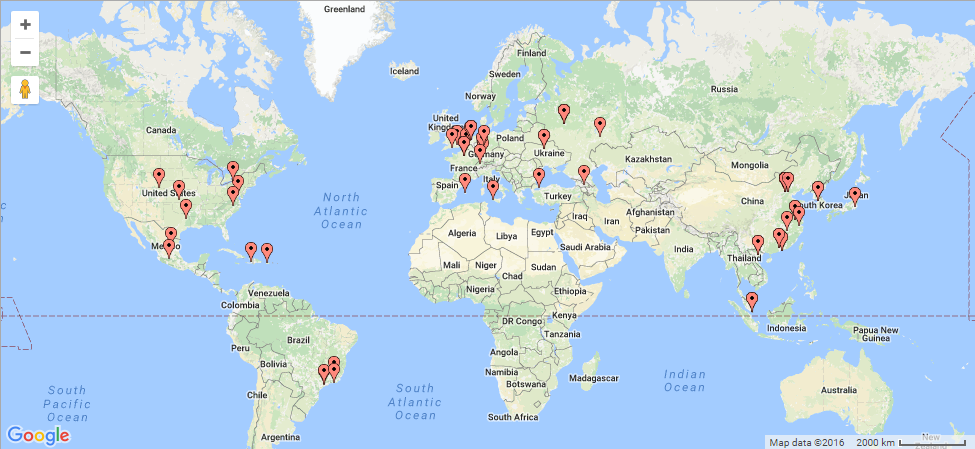
\includegraphics[width=0.94\textwidth]{img/geo_ip_world.png}
	\caption{Karte mit Geo-Location von Angreifer-IP-Adressen}
	\label{fig:geo_ip_world}
\end{figure}

Diese Karte zeigt deutliche, dass ein Großteil der Angriffe aus China, Europa und Nordamerika stammen. Abbildung \ref{fig:geo_ip_eu} zeigt speziell einen Ausschnitt von Europa:

\begin{figure}[ht]
	\centering
		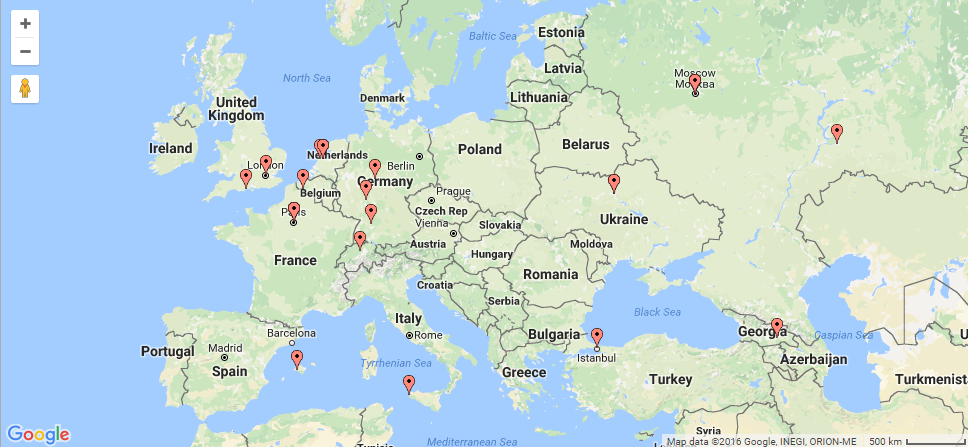
\includegraphics[width=0.94\textwidth]{img/geo_ip_eu.png}
	\caption{Karte mit Geo-Location von Angreifer-IP-Adressen}
	\label{fig:geo_ip_eu}
\end{figure}

Die Verteilung der IP-Adressen in Europa erstreckt sich hauptsächlich über Mitteleuropa. Allgemein muss diese Auswertung jedoch mit Vorsicht betrachtet werden, da die Zuordnung einer IP-Adresse zu einer Örtlichkeit einer gewissen Fehlerrate unterliegt. batchgeo.com ordnet die IP-Adresse mit Hilfe von Daten von MaxMind zu. MaxMind gibt für die Zuordnung von IP-Adressen zu Städten in Ländern wie den USA, China, Russland oder Deutschland eine Zuverlässigkeit von über 75\% an. Für andere Länder ist teilweise eine niedrigere Zuverlässigkeit gegeben, die in einigen Fällen unter 50\% liegt. Eine Auflistung je Land kann auf der Website von MaxMind\footnote{ MaxMind GeoIP2 City Accuracy: \url{https://www.maxmind.com/en/geoip2-city-database-accuracy}} eingesehen werden.



\subsection{Benachrichtigung bei Zugriff auf SSH-Honeypot}
\label{subsec:Benachrichtigung bei Zugriff auf SSH-Honeypot}

Unter \ref{sec:Kann-Kriterien} wurde eine Anforderung zur automatischen Benachrichtigung bei einem Angriff dokumentiert. Das Projektteam hat sich dazu entschieden, diese Benachrichtigung in Form einer Email-Benachrichtigung umzusetzen. Angedacht ist, eine Email dann zu versenden, wenn sich die Kippo-Logdatei ändert. Um nicht bei jeder Änderung benachrichtigt zu werden, soll in einem festen Zeitintervall auf Änderungen geprüft werden. Veränderungen an Dateien oder Verzeichnissen können unter Linux unter anderem mit \textit{inotifywait}\footnote{ \textit{inotifywait}: \url{https://linux.die.net/man/1/inotifywait}} überwacht werden. \textit{inotifywait} ist in dem Paket \textit{inotify-tools} enthalten, welches über

\begin{lstlisting}[language=bash,style=customccolor]
apt-get install inotify-tools 
\end{lstlisting}

installiert wird. Als Zeitintervall, in der auf Änderungen überprüft werden soll, wurde eine Stunde festgelegt. Dazu wird ein cronjob eingerichtet, der stündlich \textit{inotifywait} ausführt.

\begin{lstlisting}[language=bash,style=customccolor]
@hourly inotifywait -t 3599 -e modify /home/kippo/kippo/log/kippo.log && /home/dschwenk/email-alert/alert.sh
\end{lstlisting}

Als Parameter werden \textit{inotifywait} eine Zeit von 3599 Sekunden übergeben, damit sich dieser Prozess nach Ablauf dieser Zeit automatisch beendet. Würde keine Zeit angegeben werden, würde dieser Prozess bis zu einer Änderung, die in einer beliebigen Zeit in der Zukunft liegen kann, im Hintergrund weiter laufen. Stündlich würde jedoch zusätzlich ein neuer Prozess gestartet werden. Die Zeitangabe verhindert somit die Mehrfachausführung. Zusätlich wird die zu überwachende Logdatei angegeben, so wie eine Aktion, die bei einer Änderung ausgeführt werden soll. In diesem Fall soll das Skript \textit{alert.sh} ausgeführt werden, welches nachfolged aufgelistet ist:

\begin{lstlisting}[language=bash,style=customccolor]
#!/bin/bash

echo "Someone accessed our SSH honeypot running on port 22" | mailx -v \
-r "honeypot-notification@danielschwenk.de" \
-s "SSH Honeypot Notification" \
-S smtp="send.one.com" \
-S smtp-use-starttls \
-S smtp-auth=login \
-S smtp-auth-user="honeypot-notification@danielschwenk.de" \
-S smtp-auth-password="password" \
-S ssl-verify=ignore \
michael.stroh@hs-weingarten.de,daniel.schwenk@hs-weingarten.de
\end{lstlisting}

Dieses Skript sendet eine Email mit vorgegebenem Betreff und Inhalt an die beiden Projektmitglieder. Der Versand selber wird über \textit{mailx}\footnote{ \textit{mailx}: \url{https://linux.die.net/man/1/mailx}} realisiert, welches über

\begin{lstlisting}[language=bash,style=customccolor]
sudo apt-get install heirloom-mailx
\end{lstlisting}

installiert wurde. Dem \textit{mailx}-Kommando werden dazu die SMTP- und Benutzerdaten übergeben. Der Versand erfolgt mit Hilfe eines Emailaccounts, welcher beim Provider one.com\footnote{ one.com \url{https://www.one.com/de/}} angelegt wurde. Die Wahl fiel auf diesen Provider, da dieser bereits in anderen Projekten in Verwendung der Teammitglieder ist. Das in diesem Listing dargestellte Passwort wurde aus Sicherheitsgründen durch einen Platzhalter ersetzt.


\section{Web-Honeypot}
\label{sec:Web-Honeypot}

\subsection{Installation und Konfiguration SNARE}
\label{subsec:Installation und Konfiguration SNARE}

In diesem Abschnitt wird die Installation und Konfiguration eines Web-Honeypots auf Basis von SNARE beschrieben. Die Einrichtung erfolgt für Port 80 HTTP. 

\begin{lstlisting}[style=customc]
sudo apt-get install python3 python3-pip
\end{lstlisting}

Unter anderem wird Python3 für eine erfolgreiche Inbetriebnahme vorausgesetzt. Da zusätzlich noch mehrere Python-Module geladen werden müssen, bedarf es darüber hinaus des zugehörigen  Paketverwaltungsprogramms pip\footnote{ \textit{pip}: \url{https://pip.pypa.io/en/stable/}}, auch in der entsprechenden Version 3.

\begin{lstlisting}[style=customc]
pip3 install aiohttp beautifulsoup4 cssutils gitpython
\end{lstlisting}

Über das Paketverwaltungsprogramm werden daraufhin die Python-Module  installiert.

\begin{lstlisting}[style=customc]
apt-get install git
\end{lstlisting}

Falls nicht bereits systembedingt bereitgestellt, ist es an dieser Stelle zwingend erforderlich die Versionsverwaltungssoftware git\footnote{ \textit{git}: \url{https://git-scm.com/}} zu installieren.

\begin{lstlisting}[style=customc]
cd /home/mstroh/
git clone https://github.com/mushorg/snare.git
\end{lstlisting}

Über Github kann SNARE\footnote{ \textit{SNARE-Projekt auf Github}: \url{https://github.com/mushorg/snare}}: bezogen werden.

\begin{lstlisting}[style=customc]
cd /home/mstroh/snare
sudo python3 clone.py --target http://example.com
\end{lstlisting}

SNARE stellt dabei selbst ein Skript bereit um bestehende Webpräsenzen zu klonen. Diese Klone werden unter
\begin{lstlisting}[style=customc]
/opt/snare/pages
\end{lstlisting}
abgelegt. Wahlweise kann natürlich auch eine eigene Webseite erzeugt und über SNARE gestartet werden.

\begin{lstlisting}[style=customc]
sudo python3 snare.py --interface eth0 --port 80 --page-dir example.com >> snare.log &
\end{lstlisting}
Die sudo-Rechte benötigt SNARE um den Python-HTTPRequestHandler an Port 80 zu binden. Direkt nachdem das geschehen ist, werden diese Privilegien wieder abgegeben und der Web-Honeypot selbst läuft unter einem eigens hierfür angelegten nicht privilegierten Nutzer. In der Standardkonfiguration heißt dieser Nutzer nobody. Über die Parameter \grqq{}--interface\grqq{} und \grqq{}--port\grqq{} werden Interface und Port für den Web-Honeypot festgelegt. \grqq{}--page-dir\grqq{} lädt die entsprechend zuvor geklonte oder selbst erzeugte Webseite und simuliert daraufhin einen Webserver. 

Sämtliche Zugriffe, auch solche, die aufgrund einer nicht vorhandenen Ressource scheitern, Nutzer-Eingaben und Zugriffsversuche werden von SNARE über die Python-Anweisung print ausgegeben. Über \grqq{}>> snare.log\grqq{} werden diese Ausgaben an das Logfile \grqq{}snare.log\grqq{} angehängt.  Ohne weiteres Zutun würden diese Ausgaben zum jeweiligen Ereigniszeitpunkt im Zwischenspeicher der Datei \grqq{}snare.log\grqq{} verbleiben und erst bei einer größer anfallenden Menge an Log-Einträgen tatsächlich in das Log-File geschrieben werden. Um der Anforderung einer automatischen Benachrichtigung bei einem stattfindenden Angriff gerecht werden zu können, hat sich das Projektteam dazu entschlossen, die Ausgaben des Skriptes zu erweitern und den bereitgestellten Zwischenspeicher zu umgehen, um Ereignisse unmittelbar im Log-File festzuhalten und entsprechend zeitnah auf etwaige Aktivitäten reagieren zu können. 

\begin{lstlisting}[style=customc]
print(.., flush=True)
\end{lstlisting}

Das Skript wurde an entsprechenden Stellen um diesen Parameter erweitert.

\begin{figure}[ht]
	\centering
		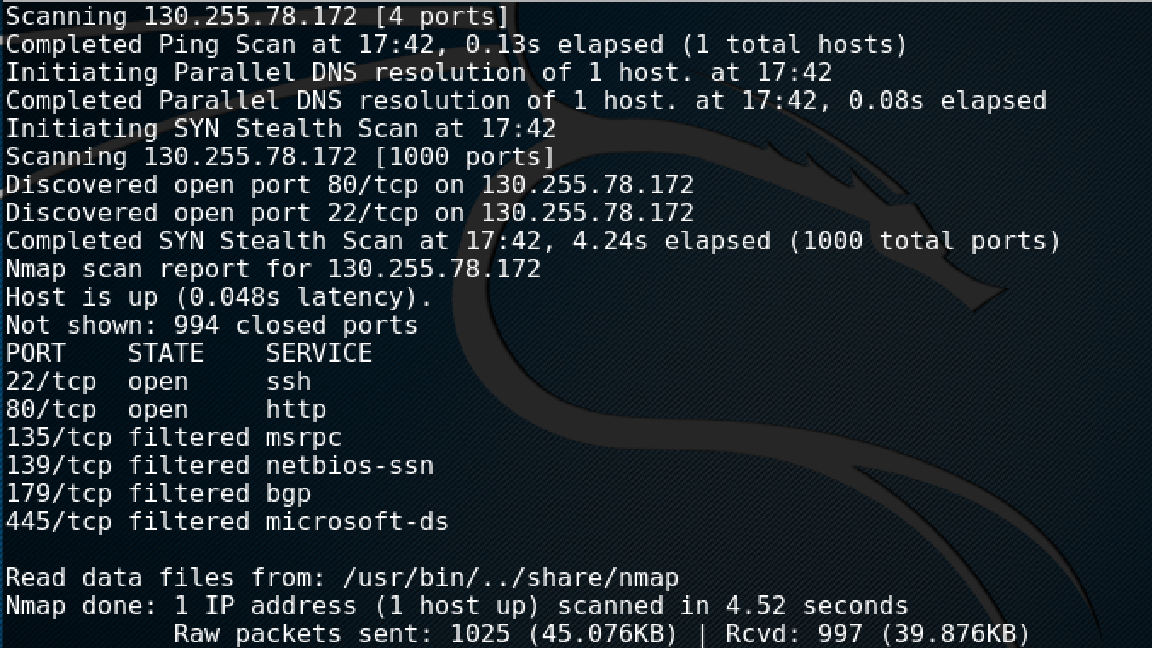
\includegraphics[width=1.0\textwidth]{img/nmap_web.png}
	\caption{Ergebnis eines Port-Scans mit Nmap nach zusätzlicher Inbetriebnahme des Web-Honeypots SNARE}
	\label{fig:nmap_web}
\end{figure}

Nach erfolgreichem Start von SNARE ist der Web-Honeypot über das zuvor angegebene Interface und den entsprechenden Port, hier 80, erreichbar.

\subsection{Verwendung eines Login-Formulars}
\label{subsec:Installation und Konfiguration SNARE}

Um einem Angreifer zusätzliche Angriffsfläche zu bieten, hat sich das Projektteam nach einwöchigem Betrieb einer Kopie von example.com\footnote{ example.com \url{http://www.example.com}} dazu entschlossen, eine Weboberfläche in Form eines Login-Formulars zu einzusetzen.

\begin{figure}[ht]
	\centering
		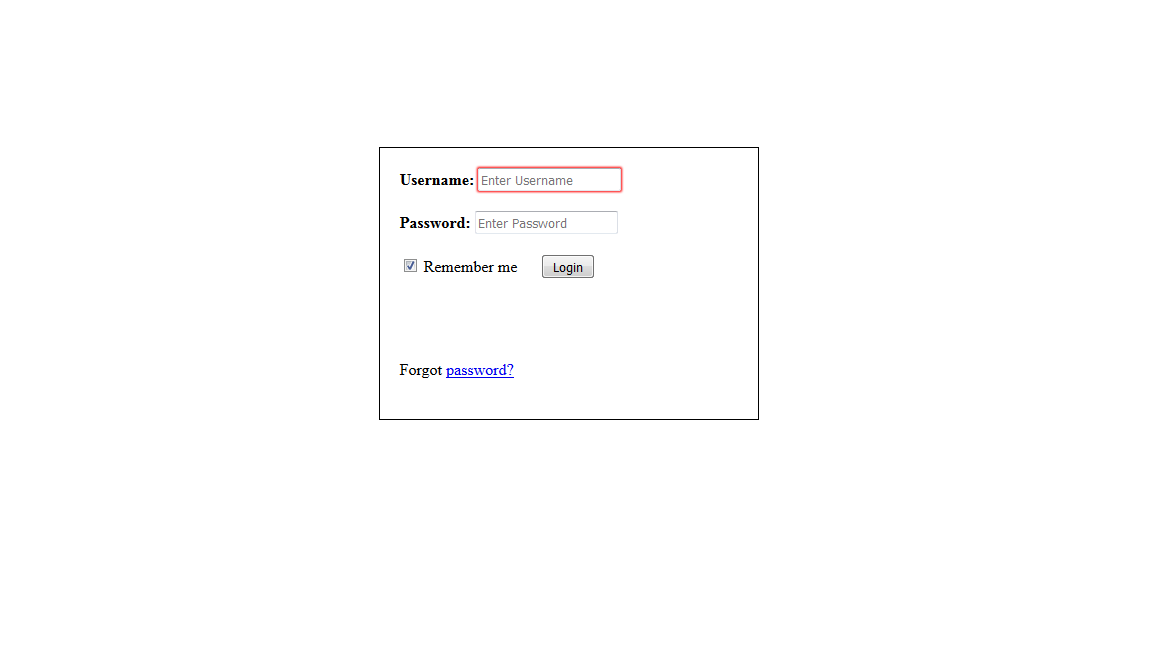
\includegraphics[width=1.0\textwidth]{img/snare_login.png}
	\caption{Weboberfläche des Web-Honeypots SNARE}
	\label{fig:snare_login}
\end{figure}

Dieses Login-Formular, wie Abbildung 6.5 ersichtlich, besteht aus lediglich zwei Eingabefeldern für jeweils Benutzername und Passwort.

\subsection{SNARE-Logfile auswerten}
\label{subsec:Installation und Konfiguration SNARE}

SNARE loggt sämtliche HTTP-Anfragen in Form des angeforderten Pfades und zusätzlich eingehende HTTP-POST-Anfragen.

\begin{figure}[ht]
	\centering
		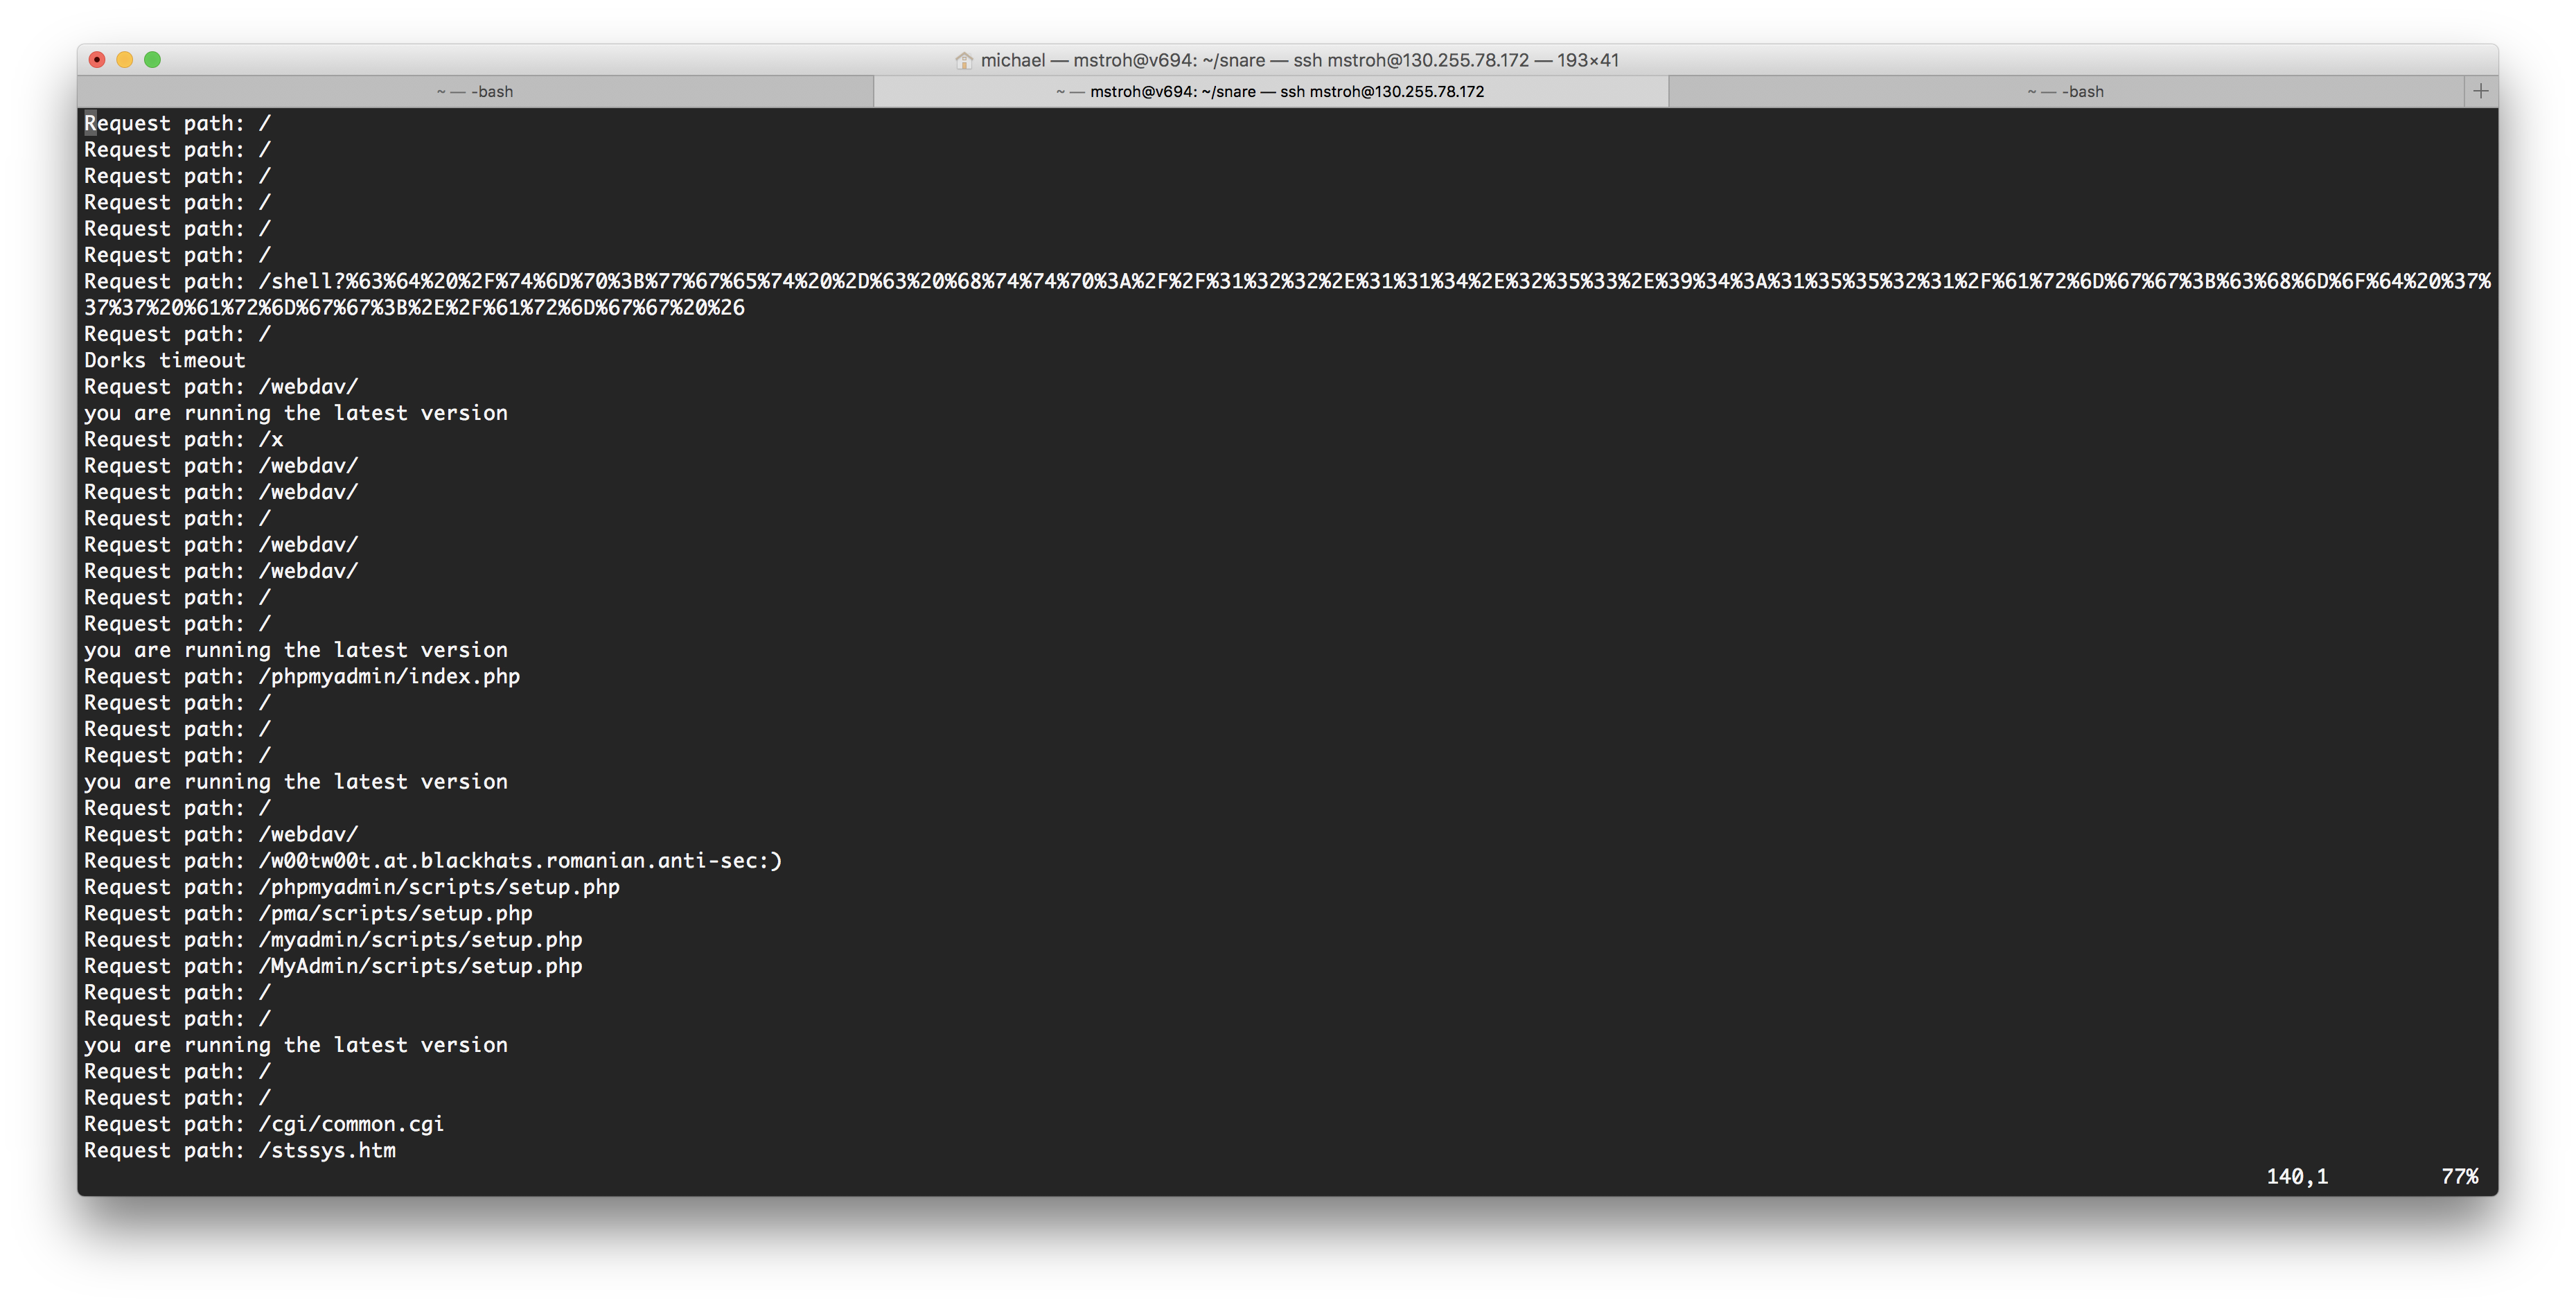
\includegraphics[width=1.0\textwidth]{img/snare_logfile.png}
	\caption{Auszug aus dem Log-File des Webhoneypots SNARE nach einwöchigem Betrieb}
	\label{fig:snare_login}
\end{figure}

Wie in Abbildung \ref{fig:snare_login} ersichtlich, werden angeforderte Pfade mit dem Präfix \grqq{}Request path:\grqq{} und POST-Anfragen mit \grqq{}POST data:\grqq{} versehen. Da zusätzliche, ebenfalls in diesem Log-File gesicherte Programm-Ausgaben, wie etwa die zum Systemstart verwendeten Parameter, für das Projektteam irrelevant sind, werden für eine weitere Unterteilung lediglich die zwei zuvor genannten Kategorien verwendet.


\begin{lstlisting}[style=customc]
grep 'POST data:' snare.log |
  sort > snare-post.txt
\end{lstlisting}

Unter Verwendung von grep werden alle Einträge, die durch einen HTTP-POST entstanden sind in eine Text-Datei geschrieben. Durch sort werden diese Einträge zudem sortiert.

\begin{lstlisting}[style=customc]
grep 'Request path:' snare.log |
  sort > snare-request-paths.txt
\end{lstlisting}

Durch die gleiche Vorgehensweise werden auch alle angeforderten Pfade extrahiert. Um eine statistische Auswertung durchführen zu können, wurde an dieser Stelle auf die Verwendung von uniq verzichtet.

TODO: Statistische Auswertung.

\subsection{Benachrichtigung bei Zugriff auf Web-Honeypot}
\label{subsec:Installation und Konfiguration SNARE}

Aufgrund von Erfahrungen bei der Verwendung einer automatischen Benachrichtigung bei dem SSH-Honeypot Kippo, hat sich das Projektteam dazu entschlossen, beim Web-Honeypot drei Mal täglich auf Veränderungen des Log-Files zu prüfen und die Projektmitglieder über neue Einträge in Kenntniss zu setzen.

TODO: Implementierung.

\section{Archivierung und Automatisierung}
\label{sec:Archivierung und Automatisierung}


\subsection{Archivierung von Daten auf Cloud-Speicher}
\label{subsec:Archivierung von Daten auf Cloud-Speicher}

Um der Soll-Anforderung nach der Archivierung von Logdaten sowie Analyseergebnisse zu entsprechen, werden diese Daten automatisiert auf einem Cloud-Speicher abgelegt. Dieses Archivierung stellt sicher, dass auf diese Daten selbst dann zurückgegriffen werden kann, wenn das System kompromittiert wurde oder nicht weiter zur Verfügung steht. Eine Marktanalyse ergibt eine Vielzahl an verfügbaren Cloud-Speichern. Das Projektteam entscheidet sich auf Grund der Verfügbarkeit eines Linux-Clients, der einfachen Installation und Konfiguration dieses Clients sowie dessen Möglichkeit zur automatischen Ausführung via Kommandozeile für Google Drive\footnote{ Google Drive: \url{https://www.google.com/intl/de_de/drive/}}. Anzumerken ist, dass dieser Client nicht von Google selbst, sondern von Petter Rasmussen in einem open source Projekt entwickelt wird\footnote{ Peter Rasmussen gDrive command line tool: \url{https://github.com/prasmussen/gdrive}}. Der Download der aktuellen Version 2.1 des 64-Bit-Clients für Linux erfolgt durch:

\begin{lstlisting}[style=customc]
wget https://docs.google.com/uc?id=0B3X9GlR6EmbnQ0FtZmJJUXEyRTA&export=download
\end{lstlisting}

Durch eine Umbennung wird der kryptische Dateiname lesbar gemacht. Zudem wird die Datei als ausführbar markiert:

\begin{lstlisting}[style=customc]
mv 0B3X9GlR6EmbnQ0FtZmJJUXEyRTA&export gdrive
chmod +x gdrive
\end{lstlisting}

Die Installation erfolgt via:

\begin{lstlisting}[style=customc]
sudo install gdrive /usr/local/bin/gdrive
\end{lstlisting}

Nach der erfolgreichen Installation des Clients müssen diesem Berechtigungen zum Zugriff auf einen Google Drive Account eingerichtet werden. Dazu wird der Client mit einem beliebigen Parameter aufgerufen:

\begin{lstlisting}[style=customc]
gdrive list
\end{lstlisting}

Infolge dessen wird eine Aufforderung zum Besuch der Google-Drive-Website zur Authentifizierung ausgegeben. Somit ist eine Verbindung zwischen dem Client und dem Google Drive-Dienst hergestellt. Das Backup selbst wird über das Skript unter \ref{subsec:Automatisierung} erstellt und hochgeladen.


\subsection{Automatisierung}
\label{subsec:Automatisierung}

In den vorherigen Kapitel wurde die Vorgehensweise zur Extraktion, Auswertung und Weiterverarbeitung von Daten erläutert. Für einzelne Aufgaben wurden dazu Skripte erstellt. Um diese Skripte nun nicht regelmäßig von Hand ausführen zu müssen, werden diese einzelne Skripte über ein zentrales Skript gesteuert und täglich ausgeführt. Dieses Skript führt folgende Aufgaben aus:

\begin{itemize}
\item Daten aus Kippo-Logdatei extrahieren
\item extrahierte Daten auswerten
\item bestehende Firewallregeln sichern sowie neue Regeln erstellen
\item x.y
\item Archivierung von Logdaten sowie Analyseergebnissen
\end{itemize}

In die Archivierung fließen sämtliche Log- und Analysedaten sowie Konfigurationsdateien ein. Dazu gehören:

\begin{itemize}
\item Kippo-Konfiguration und Logdatei
\item Auswertung der Benutzer- und Passwortdaten
\item Auswertung der IP-Adressen
\item Konfigurationsdateien von iptables
\item x.y
\end{itemize}

Für einen effizienten Upload werden die oben genannten Dateien alle 24 Stunden zu einem komprimierten zip-Archiv zusammengefasst und auf den Cloud-Speicher hochgeladen. Um diesen Vorgang zu automatisieren wird folgendes Bash-Skript angelegt:

\lstinputlisting
    [caption={Skript zur Extraktion von Benutzernamen und Passwörter aus Kippo-Logfile}
       \label{lst:mitm_onmsg},
       captionpos=b,language=bash,style=customccolor]
 {listings/do_all.sh}
 
Dieses Skript soll täglich ausgeführt werden. Dies kann über einen \textit{cronjob} erreicht werden. Da für die Konfiguration von Firewallregeln via \textit{iptbles} root-Berechtigungen notwendig sind, muss dieses Skript mit privilegierten Berechtigungen ausgeführt werden. Über \textit{sudo crontab -e} wird ein \textit{cronjob} für den root-Benutzer eingerichtet:

\begin{lstlisting}[style=customc]
@daily /home/dschwenk/do_all_stuff.sh
\end{lstlisting}

Damit wird das Skript einmal täglich ausgeführt.